% Created 2023-02-02 Thu 08:28
% Intended LaTeX compiler: lualatex
\documentclass[11pt]{article}
\usepackage{graphicx}
\usepackage{longtable}
\usepackage{wrapfig}
\usepackage{rotating}
\usepackage[normalem]{ulem}
\usepackage{amsmath}
\usepackage{amssymb}
\usepackage{capt-of}
\usepackage{hyperref}
\usepackage{minted}
\usepackage{physics}
\usepackage[margin=0.5in]{geometry}
\usepackage{minted}
\author{David Lewis}
\date{2/5/2023}
\title{Homework 1}
\hypersetup{
 pdfauthor={David Lewis},
 pdftitle={Homework 1},
 pdfkeywords={},
 pdfsubject={},
 pdfcreator={Emacs 28.2 (Org mode 9.6)}, 
 pdflang={English}}
\begin{document}

\maketitle
\section*{Task 1}
\label{sec:orga029af4}
\begin{center}

\includegraphics[width=8cm]{ubuntu-settings.jpg}
\end{center}
I followed the steps given in the assignment: I downloaded the ubuntu image from
the website, loaded it into the virtual machine, and installed ubuntu. I used
all the recommended specs given in the assignment. Additionally, I installed the
virtualbox guest tools so I could fullscreen the vm. I have done this before, so
did not run into many difficulties. The only minor difficulty was in getting
virtualbox installed in my system (NixOS), but that was easily solved by
following the directions on the NixOS wiki for virtualbox.
\section*{Task 2.1}
\label{sec:org8f4a65f}
\begin{minted}[fontsize=\scriptsize]{bash}
mkdir team_dropbox && chmod 760 team_dropbox # create directory, owner has all permissions, group has read write, others have none
\end{minted}
\section*{Task 2.2}
\label{sec:orgc87181c}
\texttt{find} is recursive by default, \texttt{.}  refers to the current directory, \texttt{-newermt}
refers to ``modified files newer than timestamp''. The time stamp is the current
date at midnight (00:00:00).
\begin{minted}[fontsize=\scriptsize]{bash}
find . -newermt "$(date +'%m/%d/%y 00:00:00')"
\end{minted}
\section*{Task 3}
\label{sec:org25937a1}
\begin{center}
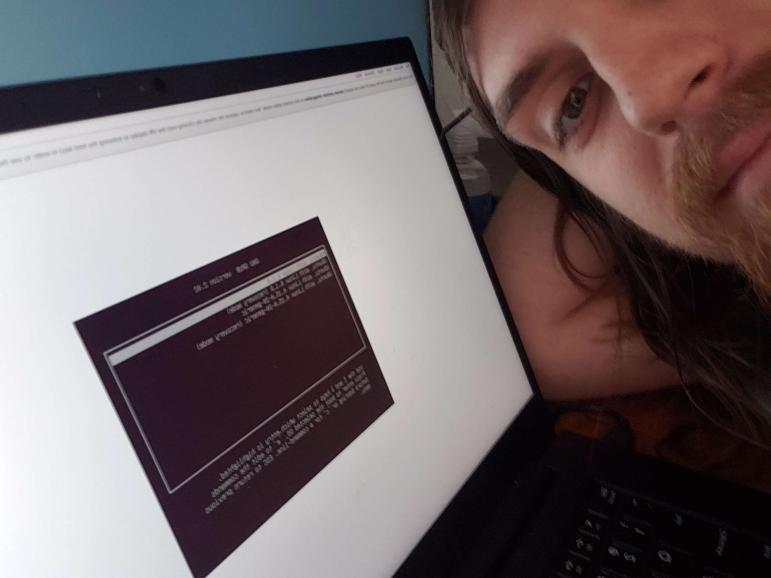
\includegraphics[width=8cm]{grub2.jpg}
\end{center}
The tutorial linked in the assignment as well as the assignment instructions are
out of date. The newest (stable) kernel is 6.1.8. The kernel listed (5.13.4) did
not seem to be available through kernel.org. None of the grub instructions were
relevant, they were all enabled by default. I did have to comment out
\texttt{GRUB\_HIDDEN\_TIMEOUT} to get the grub menu to show up, which was not in the
assignment instructions.

Also it is unclear whether or not I should have installed the kernel modules as
well as the kernel. The instructions only mentioned running make 2 times. It
would have been 3 to install the modules as well.

\section*{Task 4}
\label{sec:org608a632}
\begin{minted}[fontsize=\scriptsize]{bash}
locate -b -e 6.1.8 | grep -v /home | xargs -n 1 -p sudo rm -r && sudo update-grub
\end{minted}
This is a one-liner that removes all mention of the kernel and updates grub to
reflect the change.
\begin{itemize}
\item \texttt{locate -b -e 6.1.8}: In my case the kernel was named 6.1.8. This command
locates all files that contain 6.1.8 as a basename and also exist. This set of
files happens to be the directories where the kernel is stored.
\item \texttt{grep -v /home}: the results from locate are piped into grep, which removes the
results in the home directory. This ensures I don't delete the build directory.
\item \texttt{xargs -n 1 -p sudo rm -r}: the results from grep are piped into xargs, which
runs \texttt{sudo rm -r}, line by line, asking for permission each time.
\item \texttt{sudo update-grub}: this updates any grub related files, removing the kernel
that no longer exists.
\item No manual edits were necessary to the grub configuration (not sure why
instructions said they were needed?).
\item The only instructions needed to repeat this process is to run the one-liner in
a bash shell.
\end{itemize}
\begin{center}
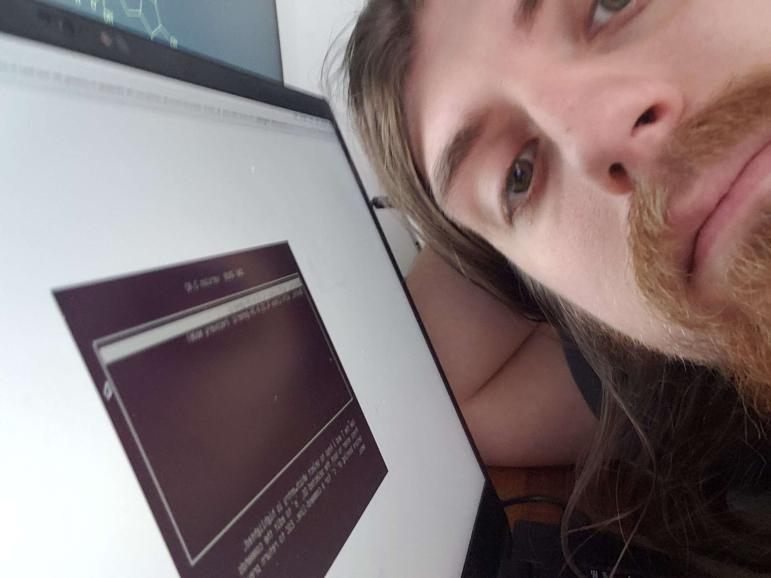
\includegraphics[width=8cm]{grub1.jpg}
\end{center}
\end{document}
